\documentclass[9pt]{beamer}

% Beamer style
%\usetheme[secheader]{Madrid}
% \usetheme{CambridgeUS}
\useoutertheme{infolines}
\usecolortheme[rgb={0.65,0.15,0.25}]{structure}
% \usefonttheme[onlymath]{serif}
\beamertemplatenavigationsymbolsempty
%\AtBeginSubsection

% Packagesg
%\usepackage[french]{babel}
\usepackage[latin1]{inputenc}
\usepackage{color}
\usepackage{xspace}
\usepackage{enumerate}
\usepackage{dsfont, stmaryrd}
% \usepackage{amsmath, amsfonts, amssymb}
\usepackage{amsmath, amsfonts, amssymb, MnSymbol}
\usepackage{epsfig}
\usepackage{tikz}
\usepackage{url}
\usepackage{/home/robin/LATEX/Biblio/astats}
%\usepackage[all]{xy}
\usepackage{graphicx}

% Commands
\input{/home/robin/RECHERCHE/EXPOSES/LATEX/Commands.tex}

% Directory
% \newcommand{\figpaper}{/home/robin/Bureau/Dropbox/VBEM-IS/Article_New/plots}
\newcommand{\fignet}{/home/robin/RECHERCHE/RESEAUX/EXPOSES/FIGURES}
\newcommand{\figtree}{/home/robin/RECHERCHE/BAYES/VBEM-IS/VBEM-IS.git/Data/Tree/Fig}
\newcommand{\figzebra}{/home/robin/RECHERCHE/BAYES/VBEM-IS/VBEM-IS.git/Data/Zebra/Fig}

%====================================================================
%====================================================================

%====================================================================
%====================================================================
\begin{document}
%====================================================================
%====================================================================

%====================================================================
\title[Bridge sampling for Poisson SBM]{Bridge sampling from deterministic approximations:  Application to the Poisson stochastic block-model}

\author[S. Robin]{S. Robin \\ ~\\
    Joint work with \underline{S. Donnet}
  }

\institute[INRA / AgroParisTech / univ. Paris Saclay]{INRA / AgroParisTech / univ. Paris Saclay
%   \vspace{-.1\textwidth}
%   \begin{tabular}{ccc}
%     
\includegraphics[height=.25\textheight]{../FIGURES/LogoINRA-Couleur} & 
%     \hspace{.02\textheight} &
%     
\includegraphics[height=.06\textheight]{../FIGURES/logagroptechsolo} % & 
% %     \hspace{.02\textheight} &
% %     
\includegraphics[height=.09\textheight]{\fignet/logo-ssb}
%     \\ 
%   \end{tabular} \\
%   \bigskip
  }

\date[November 2018, Marseille]{CIRM, Nob. 2018, Marseille}

%====================================================================
%====================================================================
\maketitle
%====================================================================

%====================================================================
%====================================================================
\section{Motivating example}
\frame{\frametitle{Outline} \tableofcontents[currentsection]}
%====================================================================
\frame{\frametitle{An ecological network}

  \paragraph{Tree network.} Set of $n$ tree species,
  $$
  \text{$Y_{ij} = $ number of (fungal) parasites hosted by both species $i$ and $j$}
  $$
  $Y = (Y_{ij}) = $ weighted adjacency matrix of the network

  \medskip 
  \paragraph{\ra Questions.}
  \begin{itemize}
   \item Does the network display some specific structure?
   \item Are there clusters of species that share more (or less) parasites?
  \end{itemize}

  \bigskip \bigskip \pause
  \paragraph{Edge covariates.} $x_{ij} = (x_{ij}^1, \dots , x_{ij}^d) = $ vector of covariates for species pair $(i, j)$:
  $$
  x_{ij} = (\text{taxonomic, geographic, genetic distance})
  $$
  
  \paragraph{\ra Questions.}
  \begin{itemize}
   \item Do these covariate contribute to structure the network?
   \item If so, are they sufficient to explain it?
   \item If there some residual structure?
  \end{itemize}
}
%====================================================================
\frame{\frametitle{Poisson stochastic block-model (SBM)}

  \paragraph{Model \refer{MRV10}.} SBM with $K$ groups
  \begin{align*}
   \{Z_i\}_i \text{ iid} & \sim  \Mcal(1, \pi) \\ 
   \{Y_{ij}\}_{i < j} \text{ independent} & \mid \{Z_i\}_i \\
   Y_{ij} \mid (Z_i=k, Z_j=\ell) & \sim \Pcal\left(\exp(\alpha_{k\ell} + \emphase{x_{ij}^\trans \beta})\right)
  \end{align*}
  
  \bigskip \pause
  \paragraph{Model parameters.} 
  \begin{itemize}
   \item $\pi = (\pi_k)_k$: group proportions
   \item $\alpha = (\alpha_{k\ell})_{k, \ell}$: interaction between groups
   \item $\beta$: effects of the covariates (regression coefficients)
  \end{itemize}
  
  \bigskip \bigskip 
  Further denote 
  $$
  Y = \{Y_{ij}\}_{i < j}, \qquad
  Z = \{Z_i\}_i, \qquad
  \theta = (\pi, \alpha, \beta).
  $$
}

% %====================================================================
% \frame{\frametitle{Outline of the talk}
% 
%   \begin{itemize}
%    \item SBM: intractable maximum likelihood inference \\ ~
%    \item Variational approximation: efficient algorithm with (almost) no statistical guaranty \\~
%    \item Side-product: approximate Fisher information \\~
%    \item Posterior sampling can take advantage of this approximate distribution
%   \end{itemize}
% }
% 
%====================================================================
\section{(Frequentist) Variational inference}
\frame{\frametitle{Outline} \tableofcontents[currentsection]}
%====================================================================
\frame{\frametitle{EM and VEM}

  SBM = incomplete data model
  
  \bigskip \bigskip
  \paragraph{Maximum likelihood.} Most popular way: EM
  $$
  \log p_\theta(Y) 
  = \Esp\left((\log p_\theta(Y, Z) \mid Y\right) - \Esp\left(\log p_\theta(Z \mid Y) \mid Y \right)
  $$
  \ra Requires to determine (some moments of) $p_\theta(Z \mid Y)$.
  
  \bigskip \bigskip \pause
  \paragraph{Variational approximation.} When $p_\theta(Z \mid Y)$ is intractable, rather maximize
  \begin{align*}
   J(\theta, q) 
   & = \log p_\theta(Y) - KL\left(q(Z) \| p_\theta(Z \mid Y) \right) \\
   & = \Esp_q\left((\log p_\theta(Y, Z)\right) - \Esp_q\left(\log p_\theta(Z \mid Y) \right)   
  \end{align*}
  taking $q \in \Qcal$. 
  
  \bigskip
  \paragraph{Mean field.} Typical choice for SBM: $\Qcal = \left\{ q: q(Z) = \prod_i q_i(Z_i) \right\}$.
  
}

%====================================================================
\frame{\frametitle{Proposed approach}

  \paragraph{VEM.}
  \begin{itemize}
   \item Popular approach for SBM avatars (i.e. weighted, including covariates or time)
%    \\ ~
   \item Few statistical guaranties (only for binary SBM without covariates) 
%    \\ ~
   \item Bayesian counterpart of VEM (VBEM) not always available
  \end{itemize}
  
  \bigskip \bigskip \pause
  \paragraph{Aim.}
  \begin{itemize}
   \item Design a posterior sampling that takes advantage of the the efficiency of VEM.
%    \\ ~
   \item Starting from frequentist inference (i.e. approximate maximum likelihood):
  $$
  (\widetilde{\theta}, \qt) = \arg\max_{\theta, q \in \Qcal} J(\theta, q)
  $$
  \end{itemize}

}

%====================================================================
\frame{\frametitle{Louis approximation}

  \paragraph{Louis formulas \refer{Lou82}.} 
  Compute Fisher information using EM side-products:
  $$
  \partial^2_{\theta^2} \log p_\theta(Y) 
  = \Esp\left(\partial^2_{\theta^2} \log p_\theta(Y, Z) \mid Y \right) 
  + \Var\left(\partial_\theta \log p_\theta(Y, Z) \mid Y \right)
  $$
  
  \bigskip \bigskip \pause
  \paragraph{Using VEM side-product.} Define the 'approximate' prior $\pt$
  $$
  \pt(\theta) = \Ncal(\theta; \widetilde{\mu}, \widetilde{\Sigma})
  $$
  where
  \begin{align*}
   \widetilde{\mu} 
   & = \widetilde{\theta} \\ ~ \\
   \widetilde{\Sigma} 
   & = \Esp_{\qt}\left(\partial^2_{\theta^2} \log p_\theta(Y, Z) \right) 
   + \Var_{\qt}\left(\partial_\theta \log p_\theta(Y, Z) \right) \\
   & \simeq \Esp_{\qt}\left(\partial^2_{\theta^2} \log p_\theta(Y, Z) \right) 
   \end{align*}
   as $\Var_{\qt}(\cdot) \simeq 0$.
}

%====================================================================
\section{Bridge sampling}
\frame{\frametitle{Outline} \tableofcontents[currentsection]}
%====================================================================
\frame{\frametitle{Bridge sampling principle}  

  \begin{tabular}{cc}
    \begin{tabular}{p{.5\textwidth}}
	 \begin{itemize}
	   \onslide+<1->{\item $\textcolor{red}{\pt} = $ proposal, $\textcolor{blue}{p^*} = $ target \\}	 
	   \onslide+<2->{\item Define intermediate distributions
		$$p_0, p_1, ..., p_H$$
		with $p_0 = q$, $p_H = p^*$ \\}	 
	   \onslide+<3->{\item Iteratively: \\
	   use $p_h$ to get a sample from $p_{h+1}$}
	 \end{itemize}
    \end{tabular}
    & 
    \hspace{-.02\textwidth}
    \begin{tabular}{p{.5\textwidth}}
 	 \begin{overprint}
 	   \onslide<1> 
 	   \includegraphics[width=.4\textwidth]{../FIGURES/FigVBEM-IS-PropTarget.pdf}
 	   \onslide<2> 
 	   \includegraphics[width=.4\textwidth]{../FIGURES/FigVBEM-IS-Tempering.pdf}
 	   \onslide<3> 
 	   \includegraphics[width=.4\textwidth]{../FIGURES/FigVBEM-IS-Tempering-step1.pdf}
 	   \onslide<4> 
 	   \includegraphics[width=.4\textwidth]{../FIGURES/FigVBEM-IS-Tempering-step2.pdf}
 	   \onslide<5> 
 	   \includegraphics[width=.4\textwidth]{../FIGURES/FigVBEM-IS-Tempering-step3.pdf}
 	   \onslide<6-> 
 	   \includegraphics[width=.4\textwidth]{../FIGURES/FigVBEM-IS-Tempering-step4.pdf}
 	 \end{overprint}
    \end{tabular}
  \end{tabular}

  \onslide+<7->{\bigskip \pause
  \paragraph{Application:}
  $$
  \pt = \pt, \qquad p^* = p(\cdot | Y)
  $$}
}
  
%====================================================================
\frame{\frametitle{Path sampling}

  Denote
  $$
  U = (\theta, Z)
  $$

  \bigskip
  \paragraph{Distribution path\footnote{\refer{Nea01}: $p_h(U) \propto \pi(U) \ell(Y | U)^{\rho_h}$, i.e. $\pt = \pi$}:} 
    set $0 = \rho_0 < \rho_1 < \dots < \rho_{H-1} < \rho_H = 1$,
  \begin{eqnarray*}
     p_h(U) & \propto & \pt(U)^{\emphase{{1-\rho_h}}} \; \times \; p(U | Y)^{\emphase{{\rho_h}}} \\
%      \\
     & \propto & \pt(U) \; \times \; \alpha(U)^{\emphase{{\rho_h}}}, \qquad  \alpha(U) = \frac{\pi(U) \ell(Y | U)}{\pt(U)}
  \end{eqnarray*}
  
  \bigskip \pause
  \paragraph{Aim of bridge sampling:} at each step $h$, provide
  $$
  \Ecal_h = \{(U_h^m, w_h^m)\}_m = \text{ weighted sample of } p_h
  $$
  
  
  \pause \bigskip 
  \paragraph{\ra Questions.}
  \begin{itemize}
   \item Step number $H$ ? Step size $\rho_h - \rho_{h-1}$?
%    \item How to actually sample $p_h$ from the \emphase{sample} $\Ecal_{h-1}$?
  \end{itemize}
}
  
%====================================================================
\frame{\frametitle{Proposed algorithm}

  \begin{description}
   \item[Init.:] Sample $(U_0^m)_m$ iid $\sim \pt$, $w_0^m = 1$ \\ ~
   \pause
   \item[Step $h$:] Using the previous sample $\Ecal_{h-1} = \{(U_{h-1}^m, w_{h-1}^m)\}$ \\ ~
   \pause
   \begin{enumerate}
    \item set $\rho_h$ such that $\emphase{cESS}(\Ecal_{h-1}; p_{h-1}, p_h) = \emphase{\tau_1}$ \\ ~
    \pause
    \item compute $w_h^m = w_{h-1}^m \times (\alpha_h^m)^{\rho_h - \rho_{h-1}}$ \\ ~
    \pause
    \item if $ESS_h = \overline{w}_h^2 / \overline{w_h^2} < \emphase{\tau_2}$, resample the particles \\ ~
    \pause
    \item propagate the particles $U_h^m \sim \emphase{K_h}(U_h^m | U_{h-1}^m)$
   \end{enumerate} ~ 
   \pause
   \item[Stop:] When $\rho_h$ reaches 1.
  \end{description}
}
  
%====================================================================
\frame{\frametitle{Some comments}

  \paragraph{Resampling (optional step 3).}
  \begin{itemize}
   \item avoids degeneracy
   \item set weights $w_h^m = 1$ after resampling 
  \end{itemize}
  
  \bigskip \bigskip 
  \paragraph{Propagation kernel $K_h$ (step 4).}
  \begin{itemize}
   \item with stationary distribution \emphase{$p_h$} (e.g. Gibbs sampler)
   \item just propagation: does not change the distribution \ra no convergence needed 
  \end{itemize}
  
  \bigskip \bigskip \pause
  \paragraph{Theoretical justification: \refer{DDJ06}.} At each step $h$, construct a distribution for the whole particle path with marginal $p_h$.

}
  
%====================================================================
\frame{\frametitle{Adaptive step size}

  \paragraph{Conditional ESS:} efficiency of sample $\Ecal$ from $q$ for distribution $p$
  $$
  cESS(\Ecal; q, p) = \frac{M \left(\sum_m W^m a^m\right)^2}{\sum_m W^m (a^m)^2}, 
  \qquad a^m = \frac{p(U^m)}{q(U^m)}
  $$
  \ra Step 1: find next $p_h$ s.t. sample $\Ecal_{h-1}$ is reasonably efficient.
  
%   \bigskip \bigskip \bigskip \pause
%   \paragraph{ESS:} intrinsic efficiency of a sample 
%   $$
%   ESS(\{(U^m, w^m)\}) = \frac{M \left(\sum_m w^m\right)^2}{\sum_m (w^m)^2}
%   $$
%   \ra Step 1c: resample if to few particles actually contribute
  
  \bigskip \bigskip \pause
  Update formula of the weights
  $$
  cESS(\Ecal_{h-1}; p_{h-1}, p_h) 
  = 
  \frac
  {M \left[\sum_m W_{h-1}^m \; (\alpha^m_{h-1})^{\rho_h -\rho_{h-1}}\right]^2}
  {\sum_m W_{h-1}^m \; (\alpha^m_{h-1})^{2\rho_h - 2\rho_{h-1}}}
  $$
  \ra can be computed for any $\rho_h$ \emphase{before sampling}.
  
  \bigskip
  \ra $\rho_h$ tuned to meet $\tau_1$, which controls the step size $\rho_h - \rho_{h-1}$ (and $H$)
}

%====================================================================
\frame{\frametitle{Marginal likelihood}

  Denote
  $$
  \gamma_h(U) = \pt(U) \alpha(U)^{\rho_h}, 
  \qquad Z_h = \int \gamma_h(U) \d U,
  \qquad p_h = \gamma_h(U) / Z_h
  $$
  
  \bigskip
  The marginal likelihood is given by
  $$
  p(Y) = \int \pi(U) \ell(Y|U) \d U = \int \gamma_H(U) \d U = Z_H
  $$

  \bigskip
  which can be estimated without bias with
  $$
  \widehat{\left(\frac{Z_H}{Z_0}\right)} = \prod_{h=1}^H \widehat{\left(\frac{Z_h}{Z_{h-1}}\right)} 
  \qquad \text{where} \quad
  \widehat{\left(\frac{Z_h}{Z_{h-1}}\right)} = \sum_m W_h^m (\alpha_h^m)^{\rho_h - \rho_{h-1}}
  $$
}
  
%====================================================================
\section{Illustrations}
\subsection*{Tree network}
\frame{\frametitle{Outline} \tableofcontents[currentsection]}

%====================================================================
\frame{\frametitle{Tree network}

  \begin{tabular}{ll}
   \begin{tabular}{p{.4\textwidth}}
    $n = 51$ species \\
    ~ \\ ~ \\
    3 covariates (distances): \\
    taxonomy, geography, genetics \\
    ~ \\ ~ \\ 
    $Y_{ij} = $ number of shared fungal parasites \\
    ~ \\

   \end{tabular}
   &
   \hspace{-.1\textwidth}
   \begin{tabular}{p{.5\textwidth}}
    \includegraphics[width=.5\textwidth]{\figtree/Tree-all-V10-M5000-net} 
   \end{tabular}
  \end{tabular}

}

%====================================================================
\frame{\frametitle{Bridge path \& choice of $K$}

  \paragraph{Full model.} All covariates

  \bigskip
  \begin{center}
    \begin{tabular}{ccc}
    $\widehat{p}(K \mid Y)$ & & Bridge path: $\rho_h$ \\
    \includegraphics[width=.3\textwidth]{\figtree/Tree-all-V10-M5000-logpY} &
    \qquad &
    \includegraphics[width=.3\textwidth]{\figtree/Tree-all-V10-M5000-rho} \\
    \textcolor{blue}{$J_K$}, \textcolor{green}{$\widetilde{BIC}$}, \textcolor{red}{$\widetilde{ICL}$} &
    \qquad &
    $\widehat{K} = \arg\max_K \widehat{p}(K \mid Y)$
    \end{tabular}
  \end{center}
}

%====================================================================
\frame{\frametitle{Posterior distribution of $\beta$}

  \begin{center}
    \begin{tabular}{ccc}
    taxonomy & geography & genetics \\
    \includegraphics[width=.3\textwidth]{\figtree/Tree-all-V10-M5000-beta1} & 
    \includegraphics[width=.3\textwidth]{\figtree/Tree-all-V10-M5000-beta2} & 
    \includegraphics[width=.3\textwidth]{\figtree/Tree-all-V10-M5000-beta3} \\
    \multicolumn{3}{c}{\textcolor{blue}{$\pt(\beta \mid \widehat{K})$}, \quad  \textcolor{red}{$\widehat{p}(\beta \mid Y, \widehat{K})$}, \quad $\widehat{p}(\beta \mid Y) = \sum_K \widehat{p}(K \mid Y) \widehat{p}(\beta \mid Y, K)$}
    \end{tabular}
  \end{center}  

  \bigskip \pause
  \hspace{-.025\textwidth}
  \begin{tabular}{rrrr}
    \paragraph{Correlation between estimates.} 
    & $(\beta_1, \beta_2)$ & $(\beta_1, \beta_3)$ & $(\beta_2, \beta_3)$ \\
    $\pt(\beta)$    & $-0.012$ & $ 0.021$ & $ 0.318$ \\
    $\widehat{p}(\beta \mid Y)$ & $-0.274$ & $-0.079$ & $-0.088$
  \end{tabular}

  \bigskip \bigskip 
  \paragraph{Model selection.} 
  $
  \widehat{P}\{\text{(taxo., geo.)} \mid Y \} \simeq 70\%, \quad
  \widehat{P}\{\text{(taxo.)} \mid Y \} \simeq 30\%
  $
}

%====================================================================
\frame{\frametitle{Residual structure}

  Between group interactions ($\alpha_{k\ell}$) = 'residuals' = not explained by the covariates.

  \pause
  \vspace{-.05\textheight} 
  \hspace{-.05\textwidth}
  \begin{tabular}{cc}
    \begin{tabular}{p{.4\textwidth}}
      \paragraph{'Graphon' representation.} \refer{LaR16} \\
      Can be represented as 
      $$
      \alpha: [0, 1]^2 \mapsto [0, 1]
      $$
      \begin{itemize}
       \item symmetric, 
       \item block-wise constant, 
       \item block width $= \pi_k - \pi_{k-1}$
       \item block height $= \alpha_{k\ell}$
      \end{itemize}
    \end{tabular}
    & 
    \hspace{-.1\textwidth}
    \begin{tabular}{p{.5\textwidth}}
      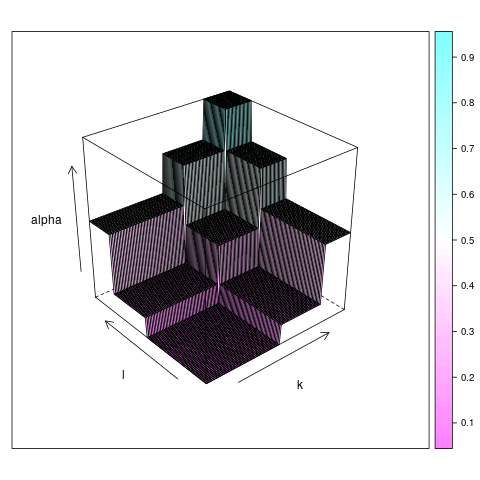
\includegraphics[width=.6\textwidth, clip=T]{\fignet/FigGraphon-SBM-graphon-alpha}
    \end{tabular}
  \end{tabular}
  
  }

%====================================================================
\frame{\frametitle{Tree network residual structure}

  \vspace{-.2\textheight}
  \hspace{-.05\textwidth}
  \begin{tabular}{cc}
    \begin{tabular}{p{.4\textwidth}}
      \paragraph{Residual graphon.} \\
      Each particule $\theta^m$ provides an estimate $\alpha^m(u, v)$ \\
      ~ \\
      ~ \\
      All estimates can be averaged (over both $m$ and $K$)
    \end{tabular}
    & 
    \hspace{-.1\textwidth}
    \begin{tabular}{p{.5\textwidth}}
    \includegraphics[width=.6\textwidth, clip=T]{\figtree/Tree-all-V10-M5000-graphon}
    \end{tabular}
  \end{tabular}
  
  \vspace{-.1\textheight}
  \paragraph{Interpretation.}
  \begin{itemize}
   \item A remaining individual effect (some species interact more than other)
   \item A small fraction of species interact much less than expected.
  \end{itemize}

}
  
%====================================================================
\subsection*{Onager networks}
%====================================================================
\frame{\frametitle{Onager social networks}

  \vspace{-.1\textheight}
  \hspace{-.05\textwidth}
  \begin{tabular}{cc}
    \begin{tabular}{p{.4\textwidth}}
      \paragraph{2 datasets.}
      \begin{itemize}
      \item $n = 28$ zebras, $n = 29$ wild asses
      \item sex and age (juvenile / adult) recorded
%       \item status = sex $\times$ age
      \end{itemize}
      
      \bigskip \bigskip 
      \paragraph{Model comparison.} \\
      Zebras: \\
      $$\widehat{P}(\text{(sex)} \mid Y) \simeq 1$$
      Wild asses: \\
      $$\widehat{P}(\text{(sex, age)} \mid Y) \simeq 1$$
%       \item status = sex $\times$ age

    \end{tabular}
    & 
    \vspace{-.2\textheight}
    \hspace{-.1\textwidth}
    \begin{tabular}{c}
    \includegraphics[width=.6\textwidth, clip=T]{\figzebra/WildAss-which-status-V10-M5000-graphon} 
    \vspace{-.1\textheight} \\
    Wild ass residual structure 
    \end{tabular}
  \end{tabular}

}
  

%====================================================================
\frame{\frametitle{Discussion}

  \paragraph{Rational.}
  \begin{itemize}
   \item Frequentist VEM side-product can be used to define approximate posterior
   \item Bridge sampling can go from there to the true posterior, avoiding MCMC convergence issues
  \end{itemize}
  
  \bigskip \bigskip \pause
  \paragraph{Some question.}
  


}
  

%====================================================================
\frame{ \frametitle{References}
{\tiny
  \bibliography{/home/robin/Biblio/BibGene}
%   \bibliographystyle{/home/robin/LATEX/Biblio/astats}
  \bibliographystyle{alpha}
  }
}

%====================================================================
\backupbegin
%====================================================================
%====================================================================
\frame{\frametitle{Theoretical justification}

  At each step $h$, \refer{DDJ06} construct a distribution for the whole particle path with marginal $p_h$. \\ ~
  
  \begin{itemize}
   \item $\overline{p}_h(\theta_{0:h})$ distribution of the particle path
   $$
   \overline{p}_h(\theta_{0:h}) \propto p_h(\theta_h) \prod_{k=1}^h L_k(\theta_{k-1} |
   \theta_k)
   $$
   \item $L_h = $ backward kernel
   $$
   L_h(\theta_{h-1} | \theta_h) = K_h(\theta_h | \theta_{h-1}) p_h(\theta_{h-1}) /
   p_h(\theta_h)
   $$
   \item Update for the weights
   $$
   w_h(\theta_{0:h}) = w_{h-1}(\theta_{0:h-1}) \alpha(\theta_h)^{\rho_h - \rho_{h-1}}
   $$
  \end{itemize}
}
  
%====================================================================
\backupend
%====================================================================

%====================================================================
%====================================================================
\end{document}
%====================================================================
%====================================================================
